% LaTeX Template for Project Report,
% It is advisable to learn the basics of LaTeX before using this template.
% A good resource to start with is http://en.wikibooks.org/wiki/LaTeX/
% Empty space after chapter/section/subsection titles can be used to insert text.
%
% Just compile this file after making all required changes.

\documentclass[12pt,a4paper]{report}
\usepackage[bookmarks, colorlinks=false, pdfborder={0 0 0}, pdftitle={Invoice Web Application}, pdfauthor={Hariharan K, Dhyan, Chirag K Deshbhandari}, pdfsubject={Project Report}, pdfkeywords={report}]{hyperref} %for creating links in the pdf version and other additional pdf attributes, no effect on the printed document


%adjust your page margins here
\usepackage[top=0.8in, bottom=0.75in, left=1.25in,right=1in]{geometry} % setting the page alignment with this package

%To change line spacing in a specific environment you will use the second way, which is to add \usepackage{setspace} to the preamble and then you can make use of the command \singlespacing, \doublespacing, or \onehalfspacing to specify the line spacing for all sections and paragraphs until you sued another command to change it.
\usepackage{setspace} 

%for page borders use this package
\usepackage{fancybox}

%use this package to change the default chapter number and name display
\usepackage{titlesec}

%for embedding images
\usepackage[pdftex]{graphicx} 

%for proper url entries
\usepackage{url} 

% Renewed commands to set the titles of various pages correctly.
\renewcommand\contentsname{\centering TABLE OF CONTENTS}
   \renewcommand\listfigurename{\centering LIST OF FIGURES}
   \renewcommand\listtablename{\centering LIST OF TABLES}
   \renewcommand\bibname{\centering REFERENCES}
   \renewcommand\appendixname{APPENDIX}

%to display chapter number left and chapter title center
\titleformat{\chapter}[display]
  {\normalfont\Large\bfseries}{\filright\chaptertitlename\ \thechapter}
  {20pt}{\Huge\filcenter}
	
\begin{document}
\renewcommand\bibname{References} %Renames "Bibliography" to "References" on ref page


\begin{titlepage}

\begin{center}
%\begin{framed}
\thispagestyle{empty}
\thisfancypage{%
  \setlength{\fboxsep}{10pt}\doublebox}{}

\vspace*{1\baselineskip}

\LARGE{\textbf{Malnad College of Engineering}} \\ 
\large{\textbf{Department of Computer Science and Engineering}}\\
\large{\textbf{Hassan - 573201, Karnataka, India}}\\[0.5cm]


\includegraphics[scale=0.7]{mce_logo.png}\\[0.5cm]
\vspace{.2in}

\Large{\small{A PROJECT REPORT \\ ON}}\\
% Title
\Large{\textsc {\textbf{``Invoice Web Application"}}}\\[0.1cm]
%Example
%\Huge{\textsc {\textbf{A case study on linux}}}\\[1.0cm]
\small \emph{Submitted in partial fulfillment of\\
        the requirements for the award of the degree of}
        \vspace{.2in}

       {\bf Bachelor of Engineering \\in\\ Computer Science and Engineering}\\[0.25cm]

\vspace{.2in}					
% Submitted by
\normalsize Submitted by \\
\begin{table}[h]
\centering
\begin{tabular}{lr}
Hariharan K & 4MC19CS050 \\
Dhyan S Agni & 4MC19CS043 \\ 
Chirag K Deshbhandari & 4MC19CS035 \\
\end{tabular}
\end{table}

\vspace{0.5cm}
Under the guidance of\\
{\textbf{Mr. Shashidhara H V}}\\
Associate Professor\\

\vspace{.2in}


% Bottom of the page
% 
\includegraphics[width=0.18\textwidth]{./mce_logo.png}\\[0.1in]
\Large{Department of Computer Science and Engineering}\\
\Large{Malnad College of Engineering}\\
\normalsize
Hassan - 573201, Karnataka, India\\
\vspace{0.2cm}
2022

%\end{framed}
\end{center}

\end{titlepage}
\newpage

\thispagestyle{empty}

\thisfancypage{%
  \setlength{\fboxsep}{10pt}\doublebox}{}
	
\vspace*{1\baselineskip}
\begin{center}

\LARGE{\textbf{Malnad College of Engineering}} \\ 
\large{\textbf{Department of Information Science and Engineering}}\\
\large{\textbf{Hassan - 573201, Karnataka, India}}\\[0.5cm]


\includegraphics[scale=0.5]{mce_logo.png}\\[0.5cm]

\emph{\LARGE Certificate}\\[1cm]
\end{center}

\normalsize This is to certify that project work entitled ``Invoice Web Application" is a bonafide work carried out by 
\begin{table}[h]
\centering
\begin{tabular}{lr}
Hariharan K & 4MC19CS050 \\
Dhyan S Agni & 4MC19CS043 \\ 
Chirag K Deshbhandari & 4MC19CS035 \\
\end{tabular}
\end{table}
in partial fulfillment for the award of  Bachelor of Engineering in Computer Science and Engineering of the Malnad College of Engineering, Hassan during the year 2021-2022.  It is certified that all corrections/suggestions indicated for Internal Assessment have been incorporated in the report deposited in the departmental library. The project report has been approved as it satisfies the academic requirements in respect of project work prescribed for the Bachelor of Engineering Degree. \\[1.0cm]

\vspace{0.25cm}

\begin{table}[h]
\centering
\begin{tabular}{lllll}
Signature of the Guide & & Signature of the HOD & & Signature of the Principal \\
\textbf{Mr. Shashidhara H V}  & & 	\textbf{Dr. Geetha Kiran A} & & \textbf{Dr. C V Venkatesh} \\ 
Associate Professor & &  Prof. \& HOD & & Principal \\
Dept. of CSE, MCE & & Dept. of CSE, MCE & & MCE
\end{tabular}
\end{table}
\vspace{0.5cm}
\begin{center}
Examiners
\end{center}
\vspace{-0.75cm}
\begin{table}[h]
\centering
\begin{tabular}{lll}
Name of the Examiner & \hspace{4cm}  & Signature of the Examiner
\end{tabular}
\end{table}
\vspace{-0.75cm}
\begin{enumerate}
\item  \vspace{0.25cm}
\item
\end{enumerate}

\newpage
\begin{center}
\thispagestyle{empty}
\vspace*{2\baselineskip}
\LARGE{\textbf{ABSTRACT}}\\[0.5cm]
\end{center}
\thispagestyle{empty}
\doublespacing
\begin{normalsize}
Invoice application being the basic need for all business, yet the software required for this purpose needs to be purchased from some software company. This creates the problem if any modifications are need to be brought to taxation methods or if any features needs to be added to meet some requirement.

Generally the invoice applications available today are just offline applications simply storing the billing info in local database. This is a drawback in the era of internet world, where people expect to get all information online regarding their purchasing details, due payments.

All the businesses irrespective of the levels of business either it may be
distributors or retailers who have wide range of customers necessarily
require an elegant and user-friendly invoice application in order for the
smooth conduction of their business. Thereby it becomes a need and
demand for an Invoice Application.

In this Invoice Web Application users first need to create their profile and then can add the items involved in their business along with the details of stocks and prices.

In this project, we have implemented a general purpose invoice web application where any user can create a profile and use it create invoices for their requirement. Since, its a web application all data and information are stored in online database server . It also has the advantage of easy updates if needed.

Whereas customers can obtain their invoices as PDF and can have trustworthy services regarding their due payments.

By the implementation of this Invoice Web Application project we can overcome the drawback of traditional invoice application and we can provide a modern general purpose invoice web application made available for any user to create invoices conveniently.
\\[1cm]
\end{normalsize}
\newpage
\vspace*{1\baselineskip}
\begin{center}
\thispagestyle{empty}
\LARGE{\textbf{ACKNOWLEDGEMENTS}}\\[1cm]
\end{center}
\vspace{0.05cm}
\doublespacing
Salutations to our beloved and highly esteemed institute ``Malnad College Of Engineering" for having well qualified staff and labs furnished with necessary equipment.

The successful completion of any task would be incomplete without mentioning the people who have constantly guided and inspired for the project and the report generation.

We avail this opportunity to thank all those people who have helped us in the whole process of completion of this project and the report.

We would like to express our deepest gratitude to our mentor {\textbf{Prof. Shashidhara H V}},Department of Computer Science and Engineering for his daily evaluation of the work and for providing us constant encouragement with his unflinching support and valuable guidance throughout this project. We are indebted to him as he has considered us worthy of this project and invested his faith in us. It was a great privilege to work under him. We will take away a lot more than just the technical knowledge from him.We would also like to place our special thanks to Dr.C V Venkatesh, Principal,Dr Geetha Kiran A,HOD Computer science and Engineering department and all Panel members Mr. Shashidhara H V(Panel Head),Associate Professor, Mr.Keerthi K S,Assistant Professor, Mr.Vasanth Kumar N.T,Assistant Professor and Mr.Ravi Kumar D,Assistant Professor,Malnad College of Engineering for providing the opportunity and the facilities for the completion of our project.\\

\large{\hspace*{3.5in} Hariharan K(4MC19CS050)}\\
\large{\hspace*{3.7in} Dhyan S Agni(4MC19CS043)}\\
\large{\hspace*{2.8in} Chirag K Deshbhandari(4MC19CS035)}\\

% Salutations to our beloved and highly esteemed institute ``Malnad College Of Engineering" for having well qualified staff and labs furnished with necessary equipment.

% The successful completion of any task would be incomplete without mentioning the people who have constantly guided and inspired for the project and the report generation.

% We avail this opportunity to thank all those people who have helped us in the whole process of completion of this project and the report.

% We would like to express our deepest gratitude to our mentor Mr. Shashidhara H V, Department of Computer Science \& Engineering for his daily evaluation of the work and for providing us constant encouragement with his unflinching support and valuable guidance throughout this project. We are indebted to him as he has considered us worthy of this project and invested his faith in us. It was a great privilege to work under him. We will take away a lot more than just the technical knowledge from him.

% We would also like to place our special thanks to Dr. C V Venkatesh, Principal, Malnad College Of Engineering for providing the opportunity and the facilities for the completion of our project. \\
\newpage



\pagenumbering{roman} %numbering before main content starts
\tableofcontents
\listoffigures
\listoftables

\newpage
\pagenumbering{arabic} %reset numbering to normal for the main content

\onehalfspacing
\chapter{Introduction}

\section{Introduction}
\subsection{Introduction to Invoice}
An invoice is a document that lists the products and 
services a business provides to a client and establishes 
an obligation on the part of the client to pay the 
business for those products and services.

Invoices are the backbone of the accounting system for 
small businesses.
\begin{figure}[h]\centering
	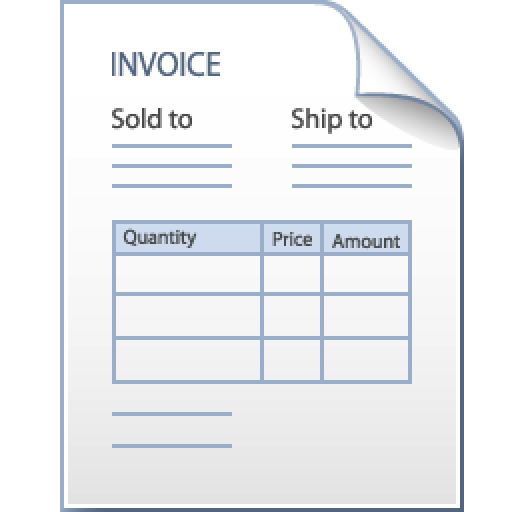
\includegraphics[width=2in]{invoice-template.png}
	\caption{A sample Invoice}\label{invoice-template}
\end{figure}

Invoices constitute some of the most valuable documents exchanged between business
partners, including government institutions. Companies exchange enormous number of
invoices daily, both in electronic and paper formats. The real obstacle lies on how efficiently and quickly the invoicing process is handled from order initiation to delivery and payment for goods or services. An invoice management system helps to simplify and
organise this process and thereby enhance process transparency.

The invoice management system generates, sorts and classifies invoices automatically.
It also monitors invoice status and sends notifications where necessary. Invoices are
automatically archived for the long term. With invoice management structures in place,
the quality of invoice data is improved.

Although invoices can be issued in a traditional printed format, e-invoicing provides methods of invoice transmission and processing via electronic means. The major difference
between e-invoices and traditional paper invoices is the automated process involved in
e-invoices.

\subsection{Problem Statement}
Invoice application being the basic need for all business, yet the software required for this purpose needs to be purchased from some software company. This creates the problem if any modifications are need to be brought to taxation methods or if any features needs to be added to meet some requirement.

Generally the invoice applications available today are just offline applications simply storing the billing info in local database. This is a drawback in the era of internet world, where people expect to get all information online regarding their purchasing details, due payments.


\section{About Project}
In this project, we have implemented a general purpose invoice web application where any user can create a profile and use it create invoices for their requirement

Since, its a web application all data and information are stored in online database server . It also has the advantage of easy updates if needed.

In this Invoice Web Application users first need to create their profile and then can add the items involved in their business along with the details of stocks and prices. 

It has features such as:
\begin{itemize}
\item Get the invoice in pdf format, which can be printed if needed.
\item Invoice history is maintained for each customer.
\item Customer details about due in their payments are maintained.
\item A copy of invoice in pdf format is sent to the customer email.\\[0.5cm]
\end{itemize}

\section{Aim and Scope}
\subsection{Aim}
To create a general purpose invoice web application where any user can conveniently utilize it to create invoices and can store all the details online and to provide modern web app features.
\subsection{Scope}
All the businesses irrespective of the levels of business either it may be distributors or retailers who have wide range of customers necessarily require an elegant and user-friendly invoice application in order for the smooth conduction of their business. Thereby it becomes a need and demand for an Invoice Application.\\[0.5cm]


\section{Objectives}
The main objective of this project is to overcome the drawback of traditional invoice application and to provide a modern general purpose invoice web application available for any user to conveniently create invoices. Also, maintain customer details to provide features regarding their due payments and invoice history. % adds the introduction page
\chapter{Literature Survey}

Invoice web application is implemented using the technologies such as
basic web components involving html, css, javascript and php\cite{webprogramming}.
Functionalities and computations involved are handled in javascript methods\cite{javascripteloquent}.
We have used some library and frameworks to implement some of features in the application.

\section{Invoice pdf generation using dompdf}
Invoices can be easily transferred to the customers if we have the generated format in PDF,to implement this feature of pdf creation of the generated invoices we have used the dompdf\cite{dompdf}.

\section{Convenient UI implemented using Bootstrap}
Being a general-purpose invoice web application has a wide category of users at different business levels. Hence, there is demand of convenient and user-friendly interface of the application which is implemented using css framework Boostrap\cite{cssbootstrap}. % adds the Literature Survey page
\chapter{Requirements}

Generally the invoice applications available today are just offline applications simply storing the billing info in local database. This is a drawback in the era of internet world, where people expect to get all information online regarding their purchasing details, due payments.

\section{System Specification}
\begin{itemize}
\item User Login and Authentication
\item Invoice Dashboard and Invoice History
\item Create Invoices
\item Update and Delete Invoices
\item Generate Invoice PDF
\end{itemize}

\section{Software Requirements}
\begin{center}
\begin{tabular}{lr}
Database & : MySQL\\
Server & : Apache\\
Text Editor & :VS Code\\
Browser & : Chrome\\
\end{tabular}
\end{center}

\chapter{Project Design}
\section{System Design}
The flow chart shown in Fig. \ref{design} is the system design representing interfaces and functional flow between interfaces used in the project.

\begin{figure}[h]\centering
	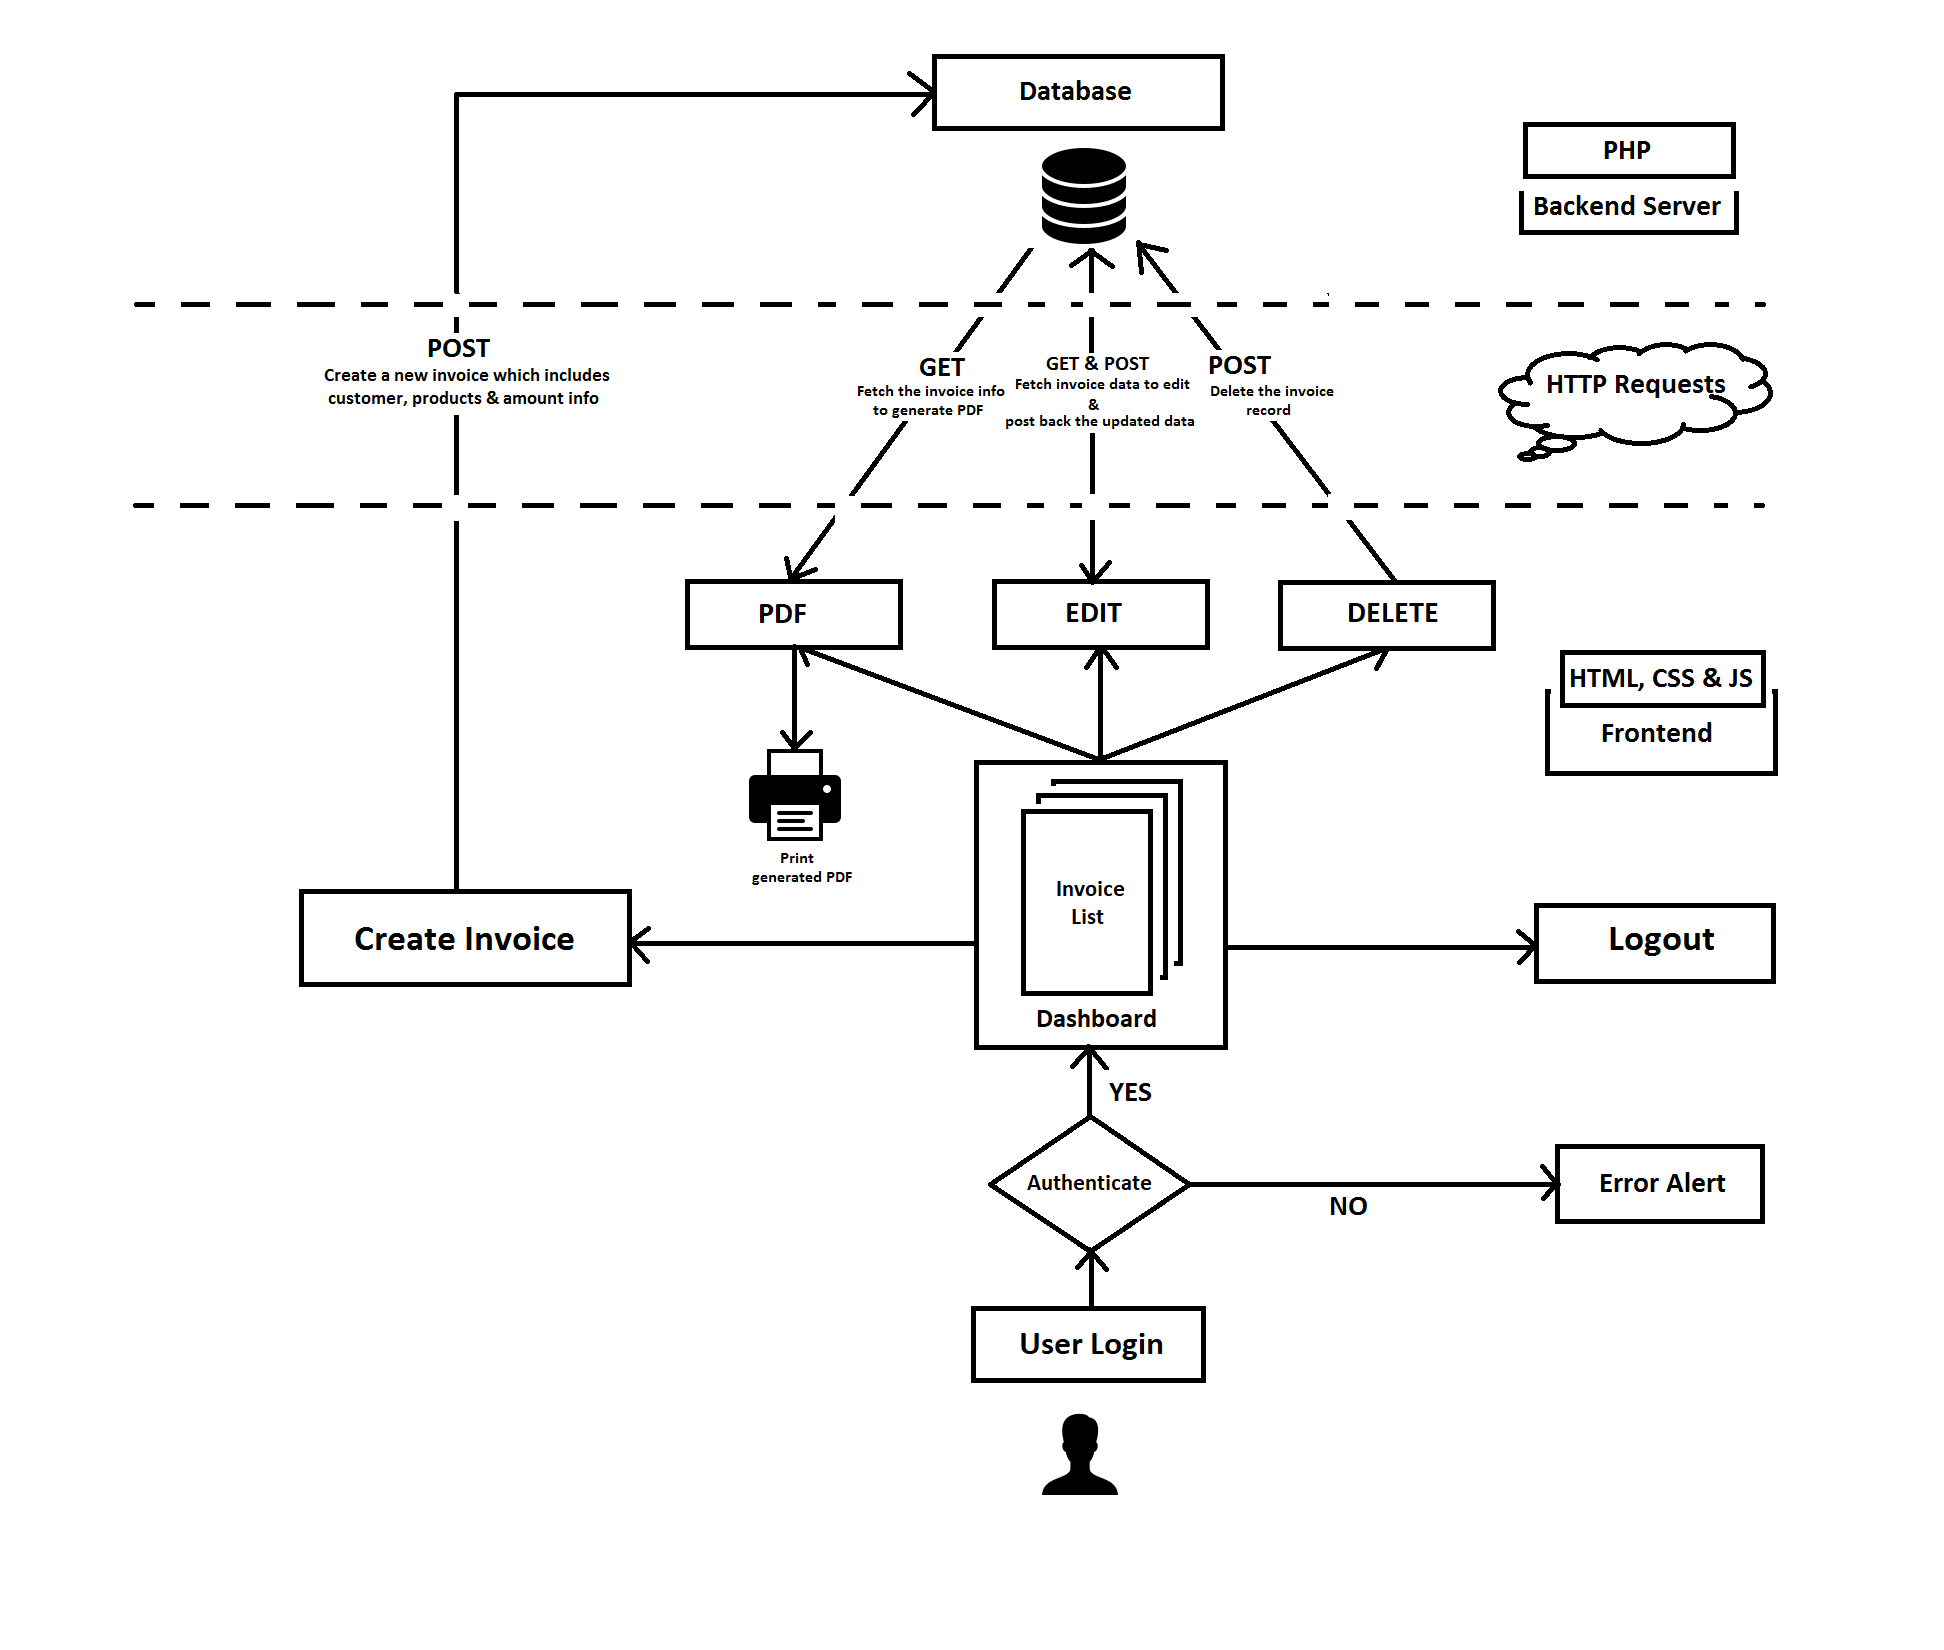
\includegraphics[width=6.5in]{design.png}
	\caption{System design of interfaces used in Invoice Web Application}\label{design}
\end{figure}
 % adds the Project Design
\chapter{Implementation}
\section{Methodology}
This web application is implemented using the technologies such as basic web components involving html, css, javascript and php. Also, we have used few web api's required to implement the invoice as pdf for easy transfer of those invoice pdf to the customers. Frameworks based on css and javascript are used to implement some functionalities wherever required.
\section{Development Tools and Technologies}
\begin{itemize}
\item \textbf{Dompdf} : dompdf is an HTML to PDF converter. At its heart, dompdf is (mostly) a CSS 2.1 compliant HTML layout and rendering engine written in PHP. It is a style-driven renderer: it will download and read external stylesheets, inline style tags, and the style attributes of individual HTML elements. It also supports most presentational HTML attributes.

Used \textbf{\textit{to implement the PDF generation}} of the invoices.

\item \textbf{Bootstrap} : Bootstrap is a free and open-source CSS framework directed at responsive, mobile-first front-end web development. It contains HTML, CSS and JavaScript-based design templates for typography, forms, buttons, navigation, and other interface components.
Used \textbf{\textit{to implement user interface convenience.}}

\end{itemize}


 % adds the implementation
\chapter{Result and Output}

\section{Result and Discussion}
We have implemented the project as a full stack Invoice Web Application with a convenient user interface focusing on ease of use for all the users since it is implemented as a general-purpose application common for any user.  

The system specifications such as User Login and Authentication, Invoice Dashboard and Invoice History, Create Invoices, Update and Delete Invoices, Generate Invoice PDF are meet while developing the system design.

The system design is developed considering the specification and requirements which is clearly representing the interfaces needed to be developed in application.

The web application is designed accordingly to the interfaces specified in the system design.This web application is implemented using the technologies such as basic web components involving html, css, javascript and php. Also, we have used few web api's required to implement the invoice as pdf and mail those invoice pdf to the customers. Frameworks based on css and javascript are used to implement some functionalities wherever required. 

Development tools like dompdf is used to implement pdf generation of the invoices.

\section{Output}

\subsection{Authentication}

\begin{figure}[h]\centering
	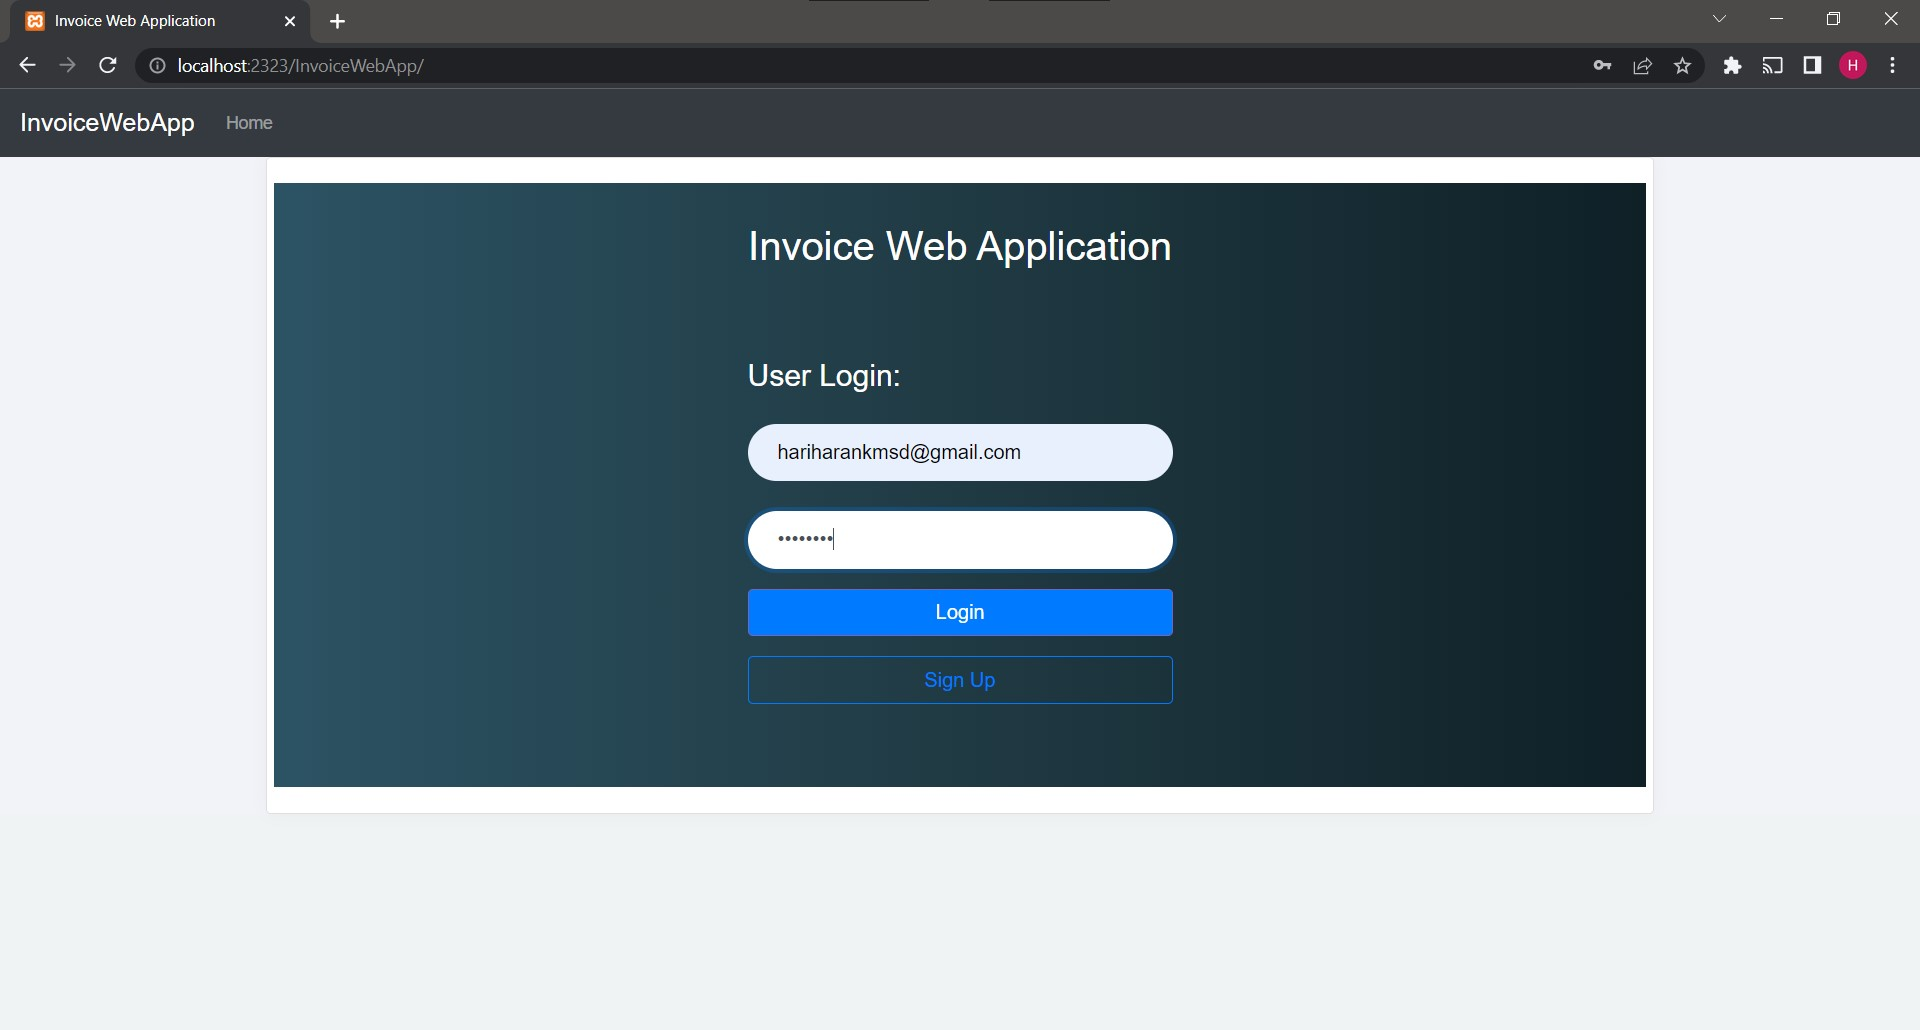
\includegraphics[width=6in]{./images/login.jpg}
	\caption{User Login Authentication Interface}\label{login}
\end{figure}



\begin{figure}[h]\centering
	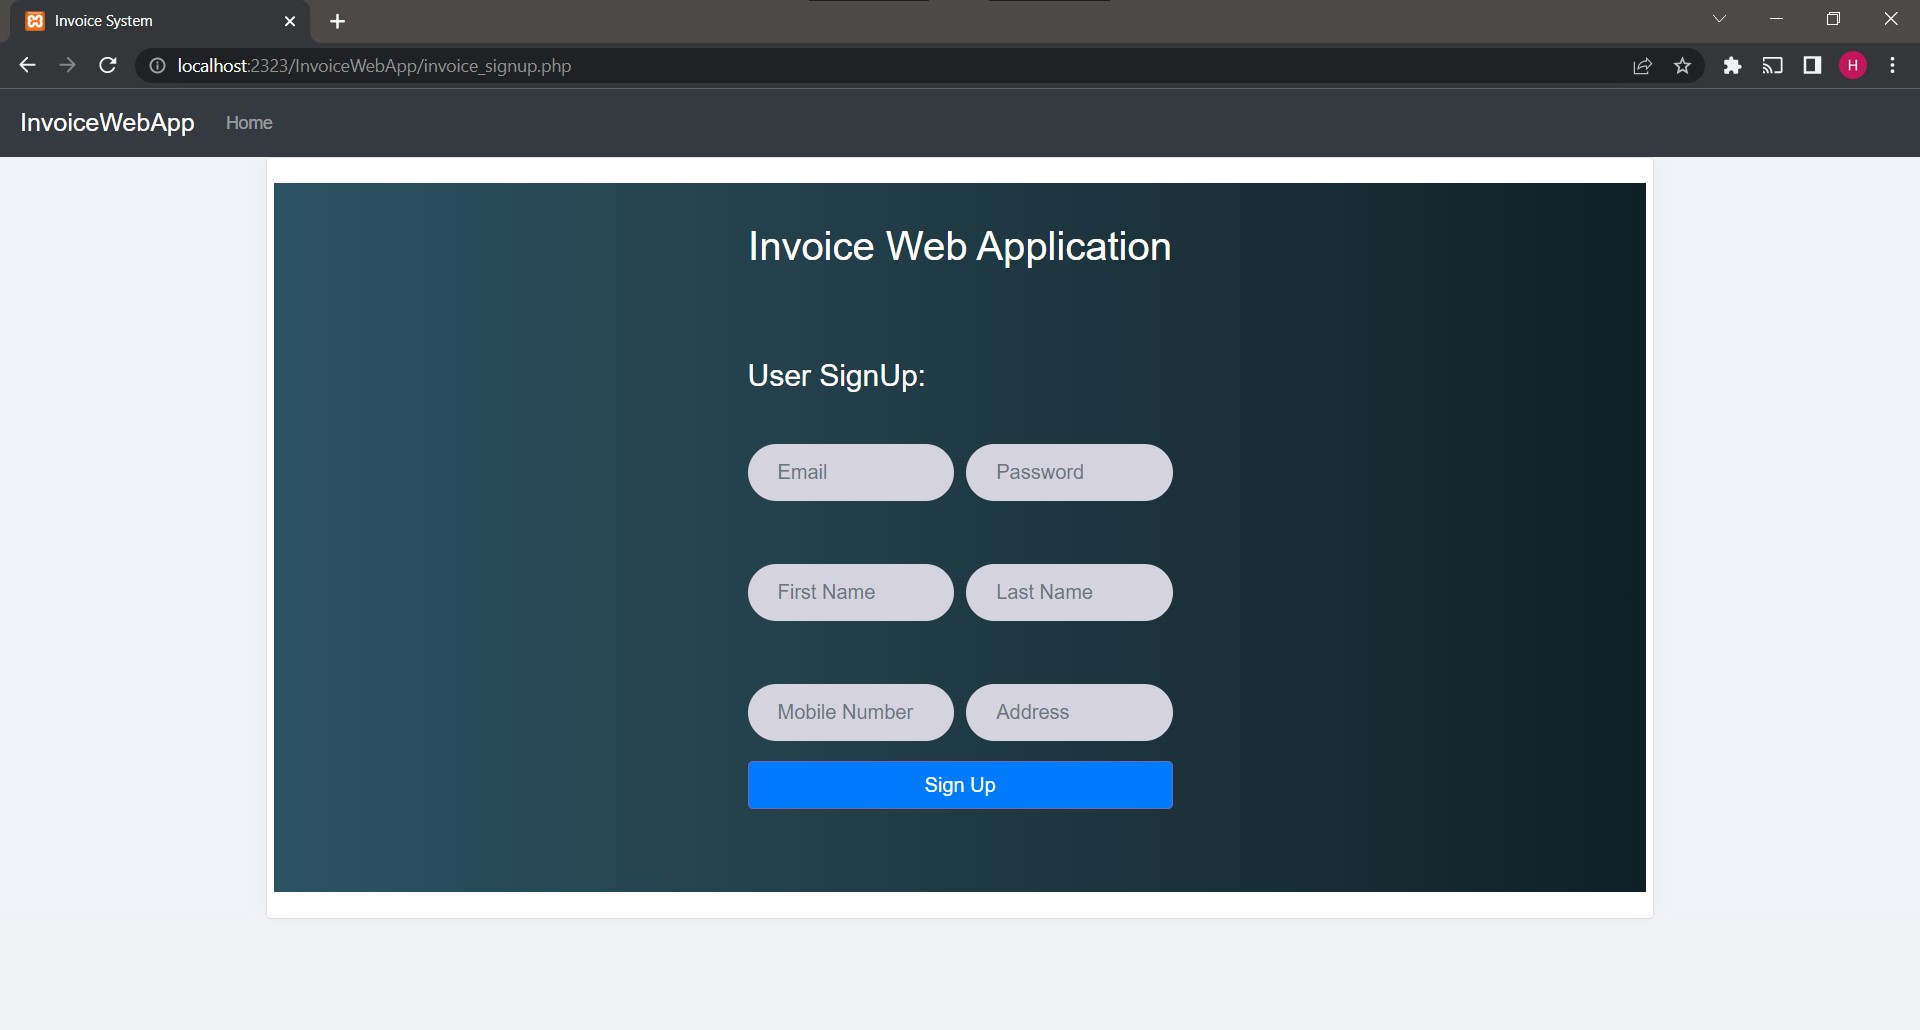
\includegraphics[width=6in]{./images/signup.jpg}
	\caption{Sign Up Interface for profile creation}\label{signup}
\end{figure}

\pagebreak

\subsection{User Interface}
\begin{figure}[h]\centering
	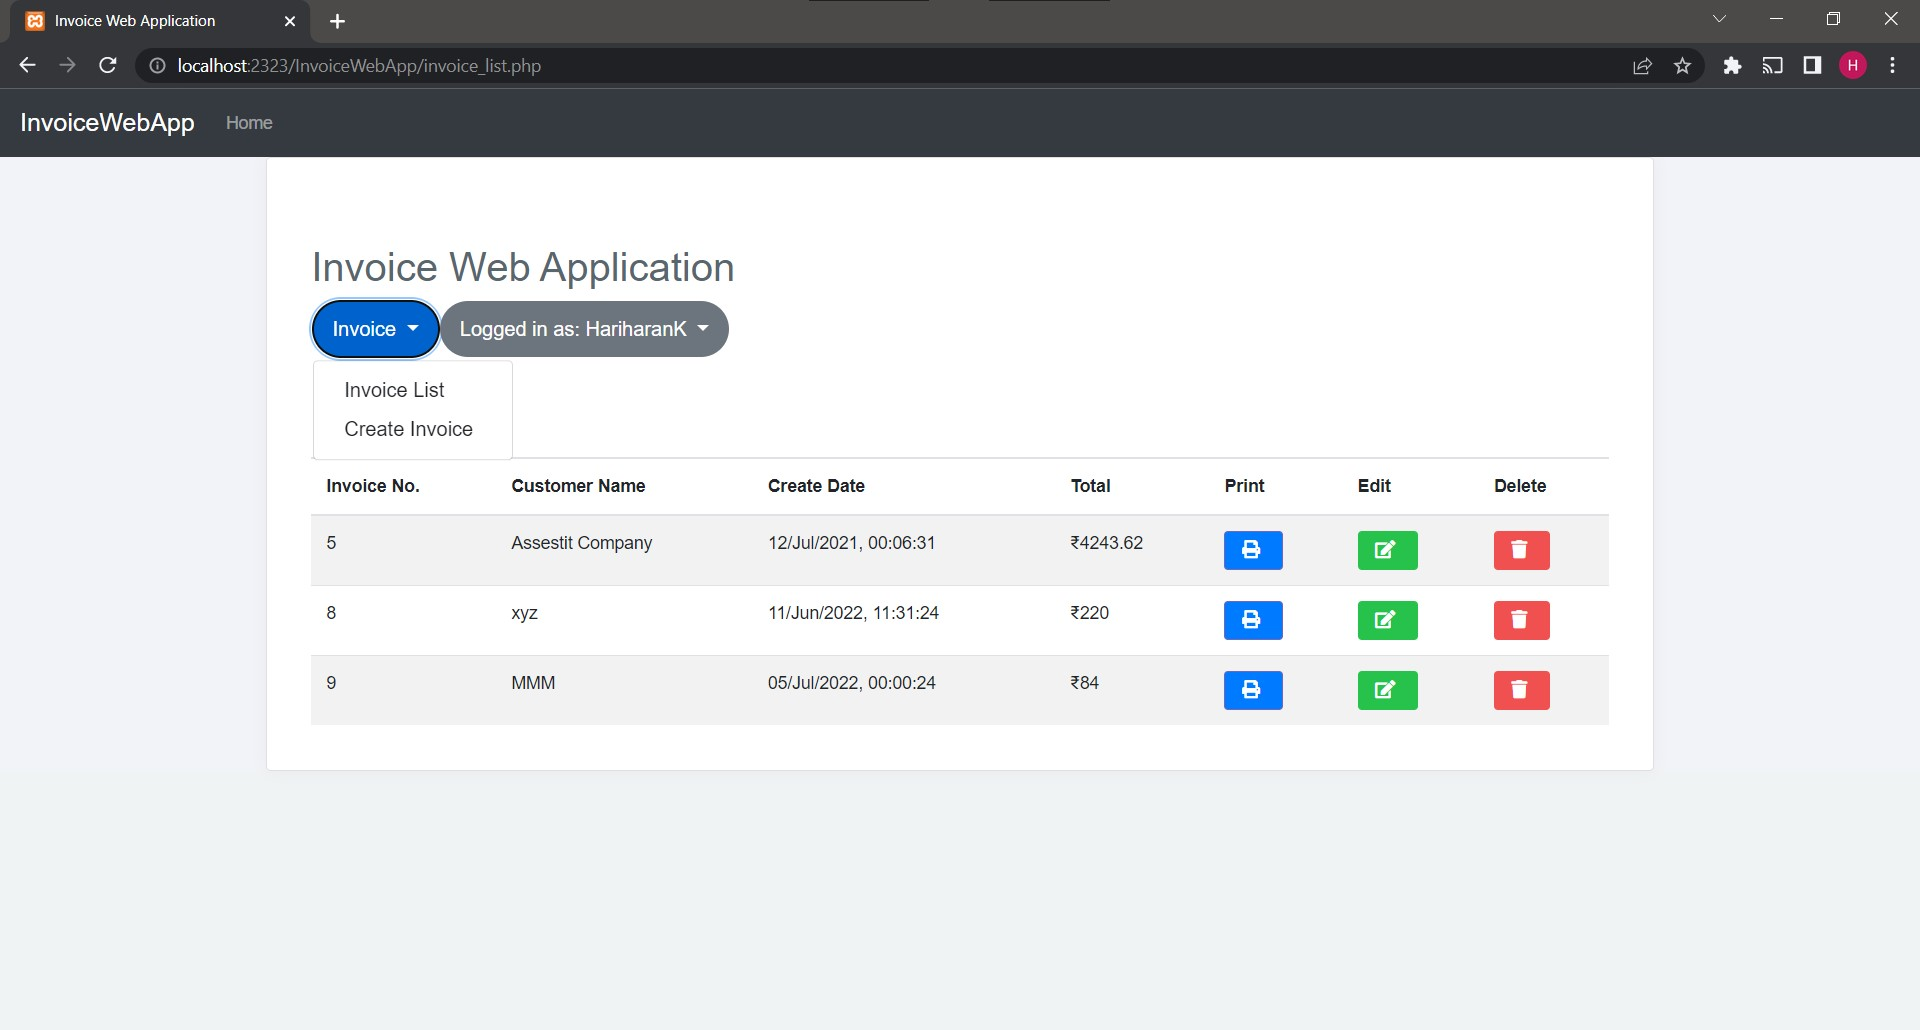
\includegraphics[width=6in]{./images/dashboard.jpg}
	\caption{Dashboard with Invoices list. Access to all other interfaces}\label{dashboard}
\end{figure}

\begin{figure}[h]\centering
	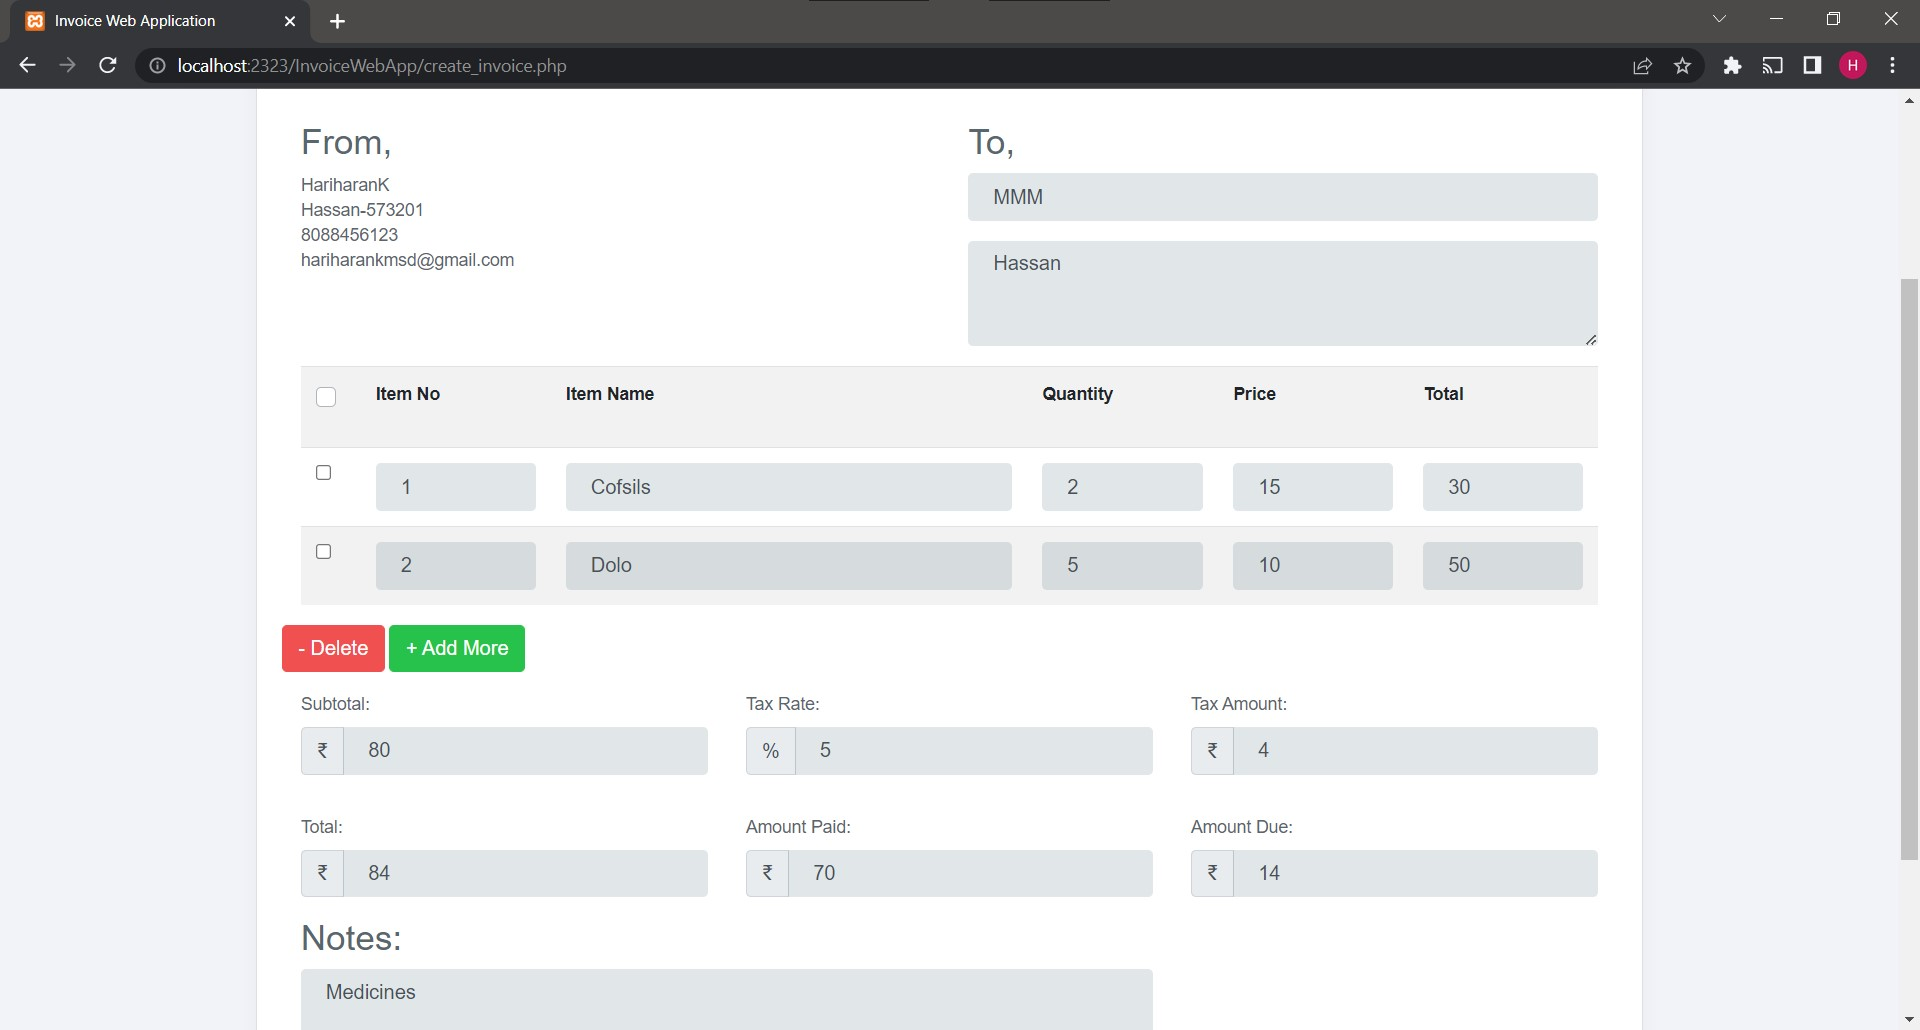
\includegraphics[width=6in]{./images/createInvoice.jpg}
	\caption{Create new invoice interface}\label{createInvoice}
\end{figure}

\pagebreak

\begin{figure}[h]\centering
	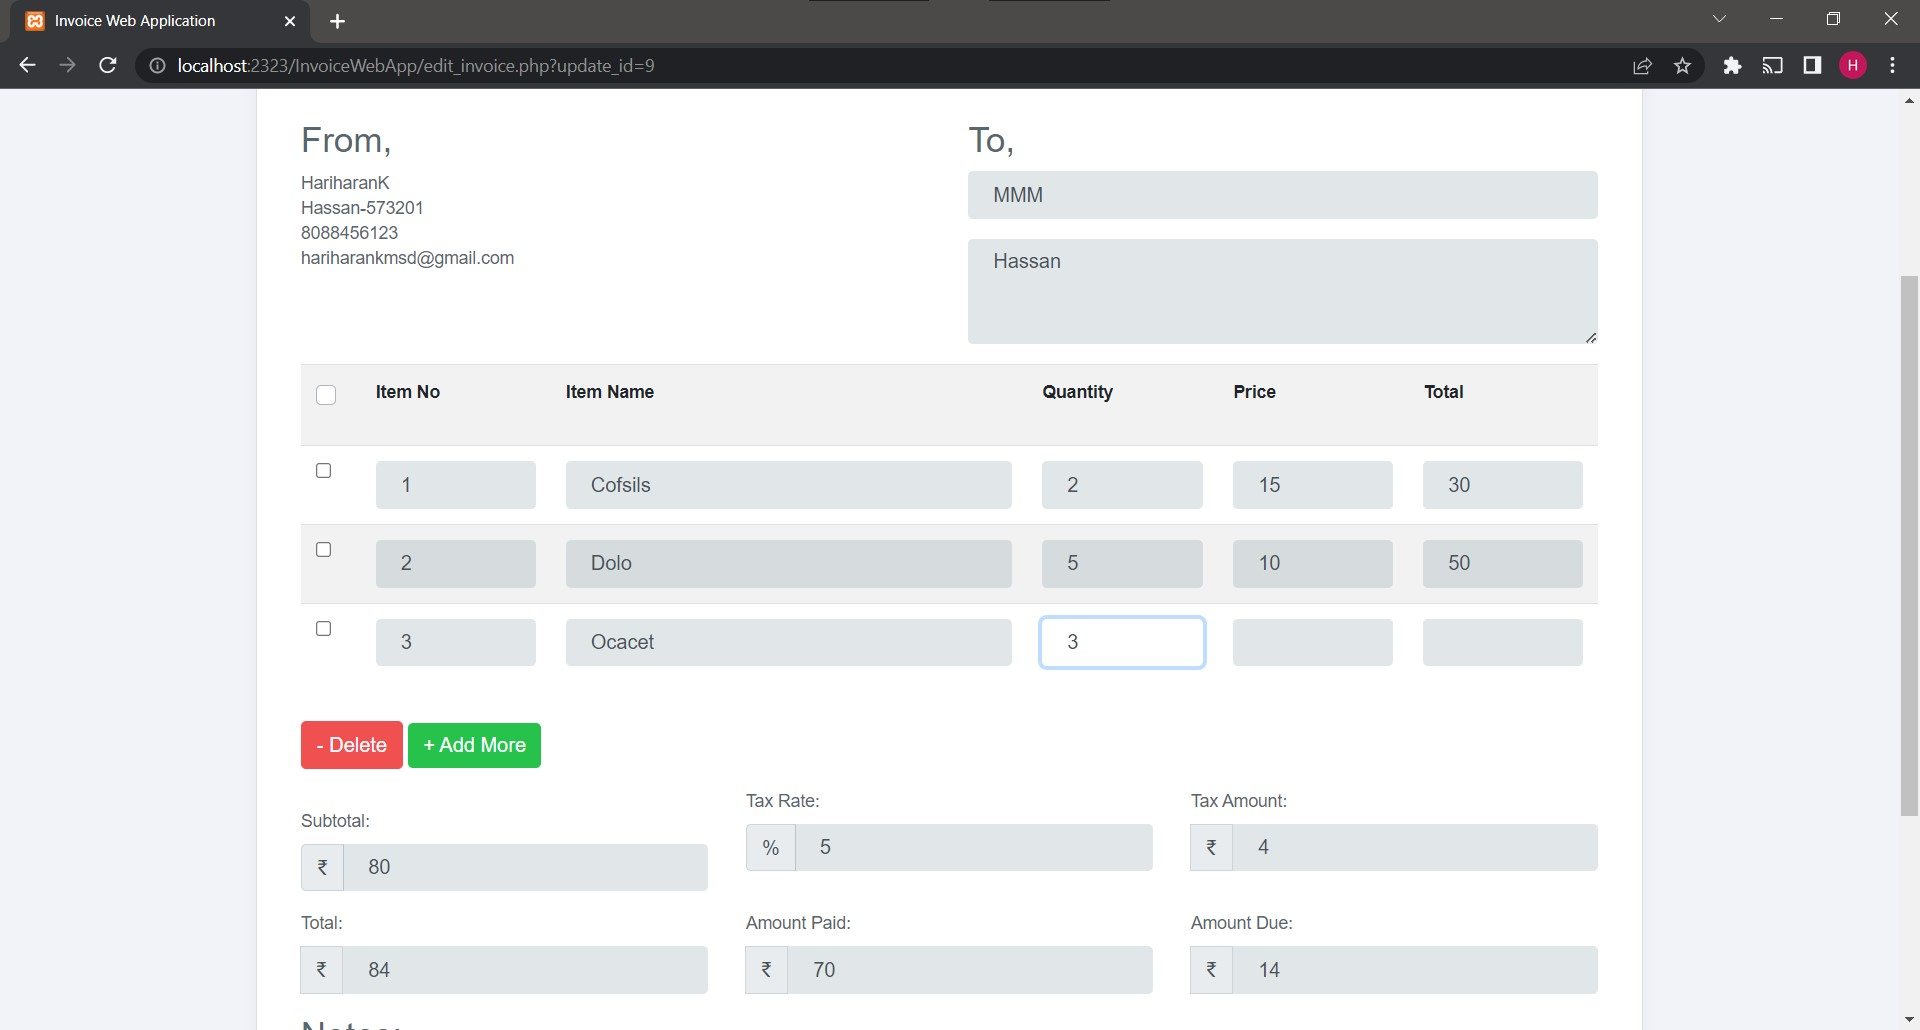
\includegraphics[width=6in]{./images/editInvoice.jpg}
	\caption{Edit existing invoices and Update the Invoice}\label{editInvoice}
\end{figure}

\begin{figure}[h]\centering
	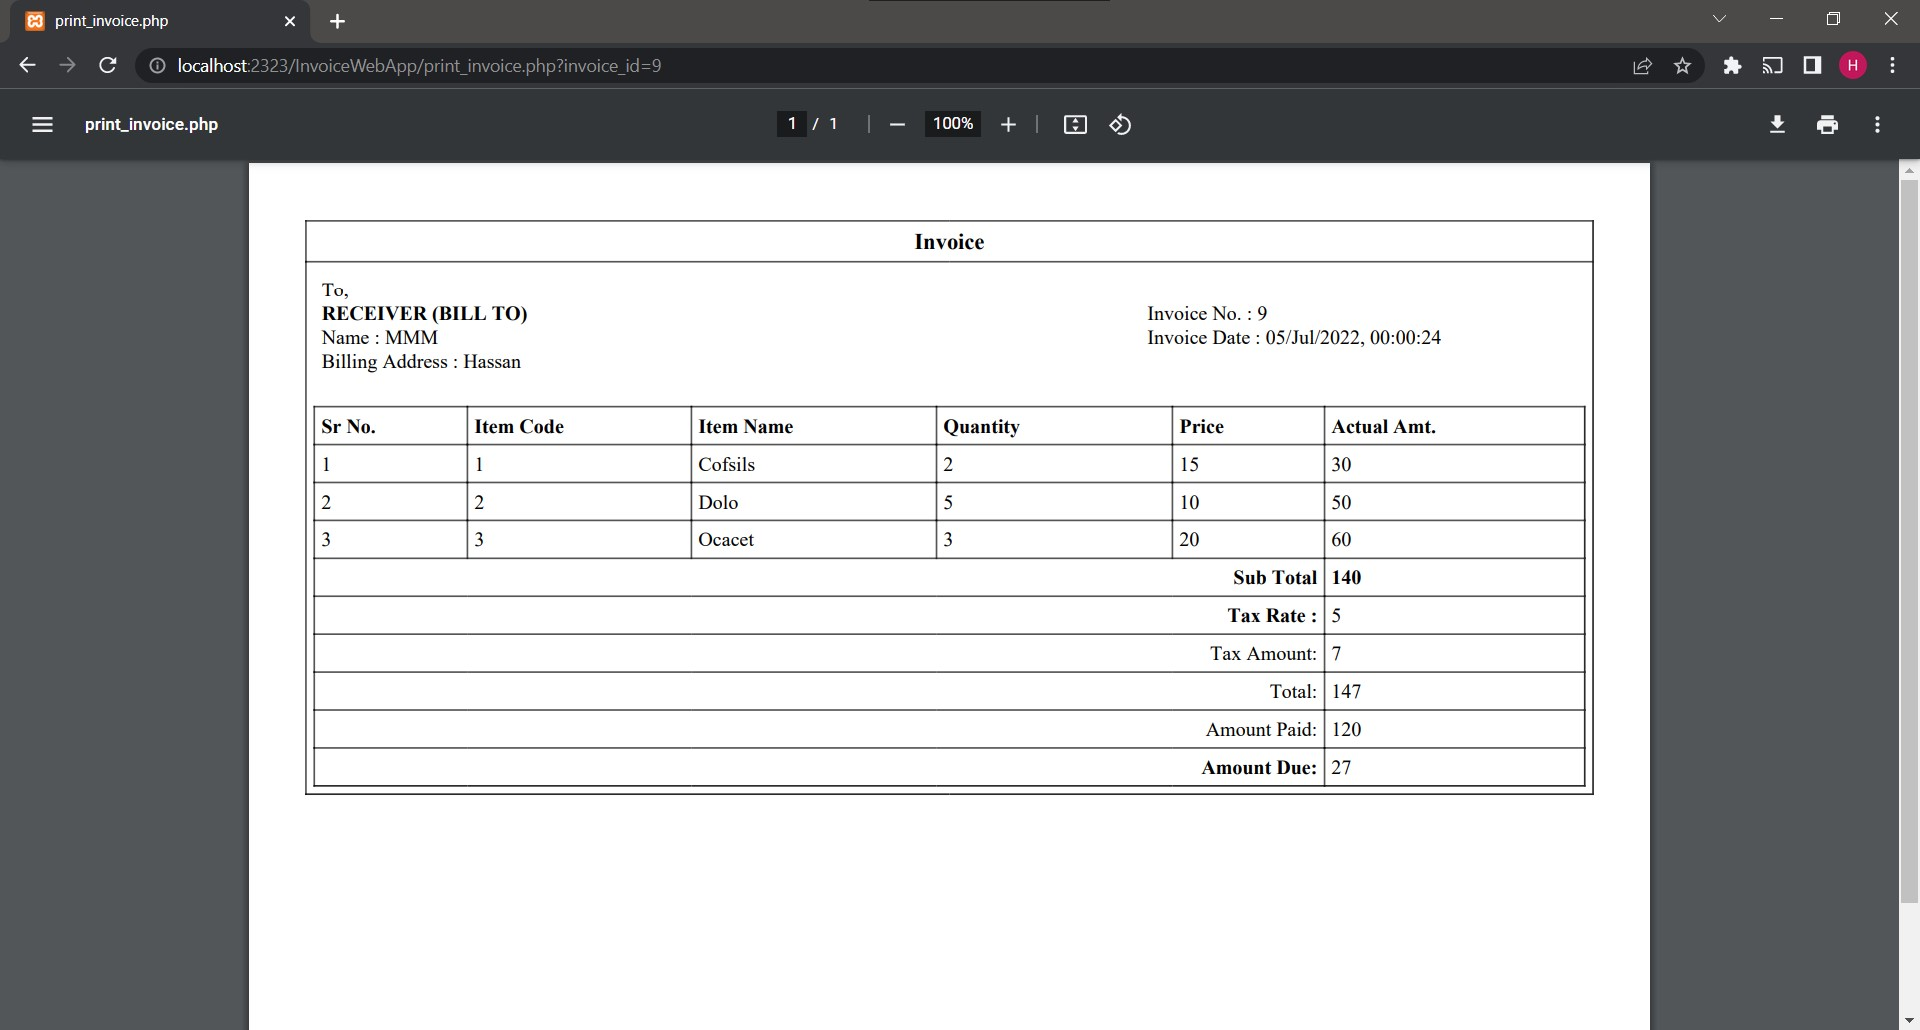
\includegraphics[width=6in]{./images/printInvoice.jpg}
	\caption{Print the invoice from generated invoice PDF}\label{printInvoice}
\end{figure}

\pagebreak

\subsection{Database Tables}

Tables list in database
\begin{table}[h]\centering
	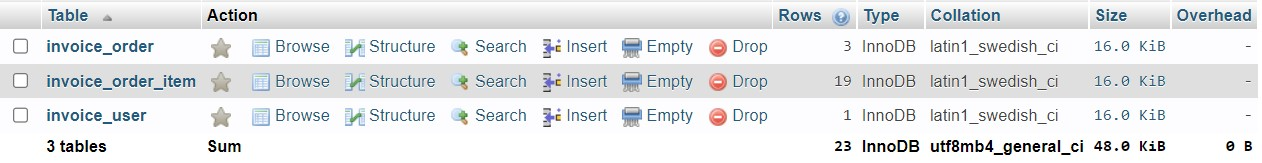
\includegraphics[width=6in]{./images/invoicetables.jpg}
	\caption{List of tables in the database}\label{invoicetables}
\end{table}

Database tables with entries 
\begin{table}[h]\centering  
    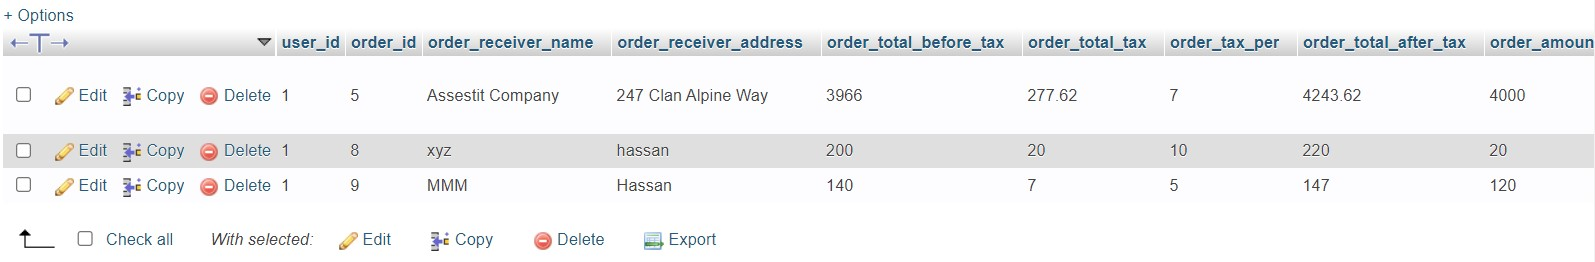
\includegraphics[width=6in]{./images/invoiceorder.jpg}
	\caption{Invoice Order table: details of each order}\label{invoiceorder}
	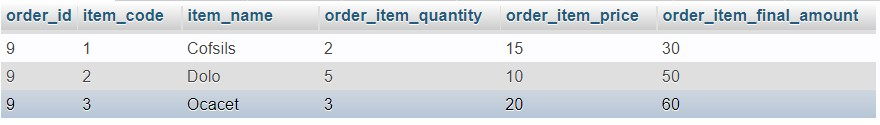
\includegraphics[width=6in]{./images/invoiceorderitem.jpg}
	\caption{Invoice Order Items table: details of items in each order}\label{invoiceorderitem}
	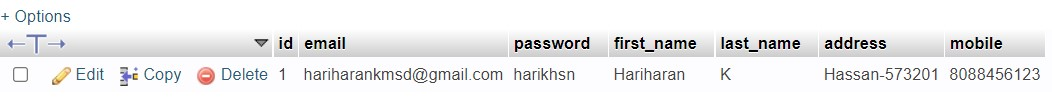
\includegraphics[width=6in]{./images/invoiceuser.jpg}
	\caption{Invoice Users table: details of user profiles}\label{invoiceuser}
\end{table}

% \begin{figure}[h]\centering
%     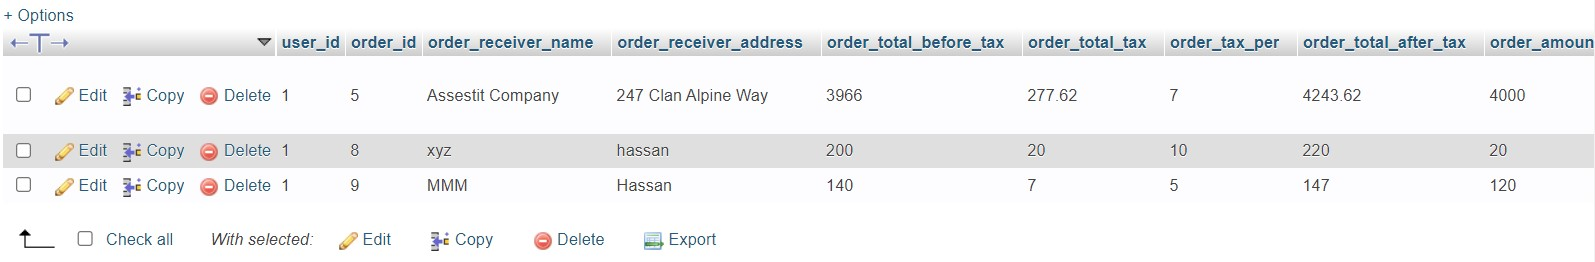
\includegraphics[width=6in]{./images/invoiceorder.jpg}
% 	\caption{Print the invoice from generated invoice PDF}\label{invoiceorder}
% 	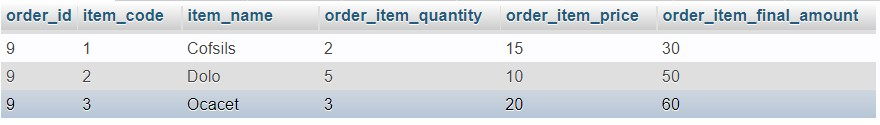
\includegraphics[width=6in]{./images/invoiceorderitem.jpg}
% 	\caption{Print the invoice from generated invoice PDF}\label{invoiceorderitem}
% 	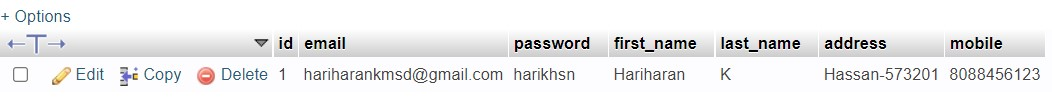
\includegraphics[width=6in]{./images/invoiceuser.jpg}
% 	\caption{Print the invoice from generated invoice PDF}\label{invoiceuser}
% \end{figure}
% \caption{Comparison of Community Detection Algorithms}\label{comp}				% adds result page
\chapter{Conclusion and Future Works}

\section{Conclusion}
In this project, we have implemented a general-purpose invoice web application, in which any user just by the creation of profile can have a web based invoice application.
Whereas customers can obtain their invoices as PDF and can have trustworthy services regarding their due payments.

Our findings are summarised as follows:
\begin{itemize}
\item Any level of business can now have a functional invoice application for their own company.
\item Invoice history keeps storing the information transaction details and due payments, helpful in proper running of business.
\item Invoices are generated as PDF which avoids traditional way of printing invoices and can transfer these invoice PDF easily to the customers. 
\item Being a web based application has the versatility of easy upgrades of features in the application whenever necessary.
\end{itemize}

\pagebreak

\section{Future Works}
The aim of the project is to overcome the limitations of traditional way of printing paper invoices. Apart from this we would like to improvise our project and consider integration of future implementation of features such as:

\begin{itemize}
\item Customisation Features
\item Customer Side Interface
\end{itemize}
General-purpose application platform requires, the need of satisfying the requirements of various range of users. Scenario where taxation methods may differ from business to business need of different feature requirement. Hence, we think of future implementations regarding the {\textbf{\textit{customisation features}}} in the application in order to satisfy various feature requirements for different set of users.

Integration of {\textbf{\textit{customer side interface}}} will be helpful directly sharing the details of invoices to the customer. Keep track of all their purchases and details regarding their due payments for each invoice. Such a customer-side interface will also be helpful in implementing online payments of their invoices. % adds conclusion page

\pagebreak
% Appendices.
 \appendix
\chapter{PDF generation code snippet}\label{code}
The following is the code snippet used to invoice as pdf using dompdf.

%Use verbatim environment to insert code
\begin{verbatim}
<?php
session_start();
include 'Invoice.php';
$invoice = new Invoice();
$invoice->checkLoggedIn();
if(!empty($_GET['invoice_id']) && $_GET['invoice_id']) {
	echo $_GET['invoice_id'];
	$invoiceValues = $invoice->getInvoice($_GET['invoice_id']);		
	$invoiceItems = $invoice->getInvoiceItems($_GET['invoice_id']);		
}
$invoiceDate=date("d/M/Y,H:i:s",
                    strtotime($invoiceValues['order_date']));
$output = '';
$output='<table width="100%" border="1" cellpadding="5" 
            cellspacing="0">
	<tr>
	<td colspan="2" align="center" style="font-size:18px"><b>Invoice</b>
	 </td>
	</tr>
	<tr>
	<td colspan="2">
	<table width="100%" cellpadding="5">
	<tr>
	<td width="65%">
	To,<br />
	<b>RECEIVER (BILL TO)</b><br />
	Name : '.$invoiceValues['order_receiver_name'].'<br /> 
	Billing Address : '.$invoiceValues['order_receiver_address'].'<br />
	</td>
	<td width="35%">         
	Invoice No. : '.$invoiceValues['order_id'].'<br />
	Invoice Date : '.$invoiceDate.'<br />
	</td>
	</tr>
	</table>
	<br />
	<table width="100%" border="1" cellpadding="5" cellspacing="0">
	<tr>
	<th align="left">Sr No.</th>
	<th align="left">Item Code</th>
	<th align="left">Item Name</th>
	<th align="left">Quantity</th>
	<th align="left">Price</th>
	<th align="left">Actual Amt.</th> 
	</tr>';
\end{verbatim}
 

\pagebreak
\addcontentsline{toc}{chapter}{References}
\begin{singlespace}
  \begin{small}
	\bibliographystyle{unsrt} %unsrt - references appear in the order in which they were cited and are labeled with numbers
	\bibliography{references}
  \end{small}
\end{singlespace}
\end{document}
